\chapter{Implementacija i korisničko sučelje}
		
		
		\section{Korištene tehnologije i alati}
		
			\textbf{\textit{dio 2. revizije}}
			
			 \textit{Detaljno navesti sve tehnologije i alate koji su primijenjeni pri izradi dokumentacije i aplikacije. Ukratko ih opisati, te navesti njihovo značenje i mjesto primjene. Za svaki navedeni alat i tehnologiju je potrebno \textbf{navesti internet poveznicu} gdje se mogu preuzeti ili više saznati o njima}.
			 
			 Komunikacija u timu realizirana je korištenjem aplikacija \underline{Whatsapp}\footnote{\url{https://www.whatsapp.com/}} i \underline{Discord}\footnote{\url{https://discord.com/}}. Pri izradu raznih dijagrama kao što su dijagram razreda, dijagram komponenti, dijagram razmještaja, sekvenvijski dijagram itd. korišten je alat \underline{Astah-UML}\footnote{\url{https://astah.net/products/astah-uml/}}.
			 Za upravljanje izvornim kodom korišten je \underline{Git}\footnote{\url{https://git-scm.com/}}, a udaljeni repozitorij projekta nalazi se na platformi \underline{GitLab}\footnote{\url{https://about.gitlab.com/}}.
			 Kao razvojno okruženje korišten je \underline{Visual Studio Code} \footnote{\url{https://code.visualstudio.com/}} koji je napravio Microsoft. VSC se koristi pri izradi web-aplikacija, web-stranica, ali i mobilnih aplikacija.
			 \textit{Backend} naše web-aplikacije napisan je u programskom jeziku \underline{Java} \footnote{\url{https://www.java.com/en/}} u \underline{Intellij}\footnote{\url{https://www.jetbrains.com/idea/}} razvojnom okruženju dok je \textit{frontend} napisan u VSC-u pomoću HTML-a i CSS-a. Baza podataka nalazi se na \underline{PostgreSQL-u}\footnote{\url{https://www.postgresql.org/}}, tj. korišten je \underline{pgAdmin}\footnote{\url{https://www.pgadmin.org/}} koji je dio postgreSQL-a. Za \textit{deploy} aplikacije korišten je servis \underline{Heroku}\footnote{\url{https://www.heroku.com/}} koji podržava Javu kao programski jezik. \underline{Tesseract OCR}\footnote{\url{https://github.com/tesseract-ocr/tesseract}} smo koristili kako bi implementirali OCR.
			
			\eject 
		
	
		\section{Ispitivanje programskog rješenja}
			
			\textbf{\textit{dio 2. revizije}}\\
			
			 \textit{U ovom poglavlju je potrebno opisati provedbu ispitivanja implementiranih funkcionalnosti na razini komponenti i na razini cijelog sustava s prikazom odabranih ispitnih slučajeva. Studenti trebaju ispitati temeljnu funkcionalnost i rubne uvjete.}
	
			
			\subsection{Ispitivanje komponenti}
			\textit{Potrebno je provesti ispitivanje jedinica (engl. unit testing) nad razredima koji implementiraju temeljne funkcionalnosti. Razraditi \textbf{minimalno 6 ispitnih slučajeva} u kojima će se ispitati redovni slučajevi, rubni uvjeti te izazivanje pogreške (engl. exception throwing). Poželjno je stvoriti i ispitni slučaj koji koristi funkcionalnosti koje nisu implementirane. Potrebno je priložiti izvorni kôd svih ispitnih slučajeva te prikaz rezultata izvođenja ispita u razvojnom okruženju (prolaz/pad ispita). }
			
			
			
			\subsection{Ispitivanje sustava}
			
			 \textit{Potrebno je provesti i opisati ispitivanje sustava koristeći radni okvir Selenium\footnote{\url{https://www.seleniumhq.org/}}. Razraditi \textbf{minimalno 4 ispitna slučaja} u kojima će se ispitati redovni slučajevi, rubni uvjeti te poziv funkcionalnosti koja nije implementirana/izaziva pogrešku kako bi se vidjelo na koji način sustav reagira kada nešto nije u potpunosti ostvareno. Ispitni slučaj se treba sastojati od ulaza (npr. korisničko ime i lozinka), očekivanog izlaza ili rezultata, koraka ispitivanja i dobivenog izlaza ili rezultata.\\ }
			 
			 \textit{Izradu ispitnih slučajeva pomoću radnog okvira Selenium moguće je provesti pomoću jednog od sljedeća dva alata:}
			 \begin{itemize}
			 	\item \textit{dodatak za preglednik \textbf{Selenium IDE} - snimanje korisnikovih akcija radi automatskog ponavljanja ispita	}
			 	\item \textit{\textbf{Selenium WebDriver} - podrška za pisanje ispita u jezicima Java, C\#, PHP koristeći posebno programsko sučelje.}
			 \end{itemize}
		 	\textit{Detalji o korištenju alata Selenium bit će prikazani na posebnom predavanju tijekom semestra.}
			
			\eject 
		
		
		\section{Dijagram razmještaja}
			
			\textbf{\textit{dio 2. revizije}}
			
			 \textit{Potrebno je umetnuti \textbf{specifikacijski} dijagram razmještaja i opisati ga. Moguće je umjesto specifikacijskog dijagrama razmještaja umetnuti dijagram razmještaja instanci, pod uvjetom da taj dijagram bolje opisuje neki važniji dio sustava.}
			
			\eject 
		
		\section{Upute za puštanje u pogon}
		
				
			 \text Kada je gotov izvorni kod, može se prijeći na puštanje aplikacije u pogon. Aplikaciju smo pustili u pogon preko besplatne platforme za implementaciju aplikacije \textbf{Heroku}. Prvo je potrebno napraviti korisnički račun na web stranici : https://www.heroku.com/. Nakon uspješnog kreiranja računa ulazi se u svoj račun, klikom odaberemo u gornjem desnom kutu tipku "New" iz koje će nam se ponuditi u izborniku "New app" i "New pipeline", mi odabiremo "New app".
			 
			 \begin{figure}[H]
			 	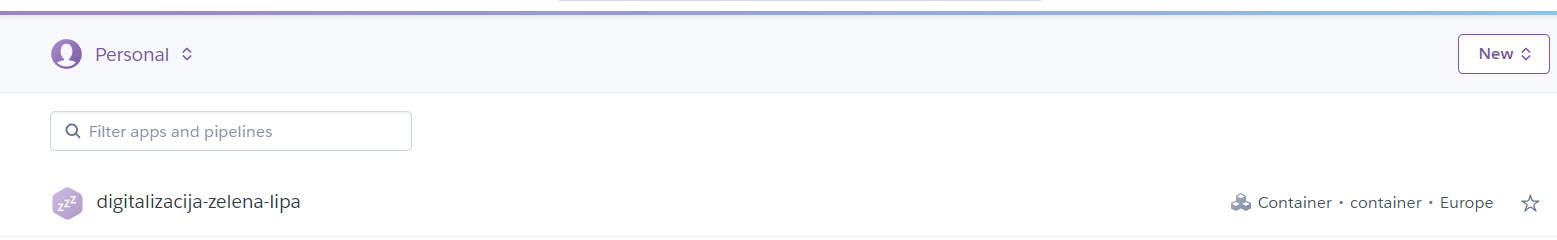
\includegraphics[scale=0.5]{slike/odabir aplikacije.png} 
			 	\centering
			 	\caption{Početna stranica/ Odabir aplikacije}
			 	\label{DS}
			 \end{figure}
			 
			 Nakon toga se na novom prozoru upisuje ime aplikacije i odabire se regija (preporučujemo Europa.)
			 
			 \begin{figure}[H]
			 	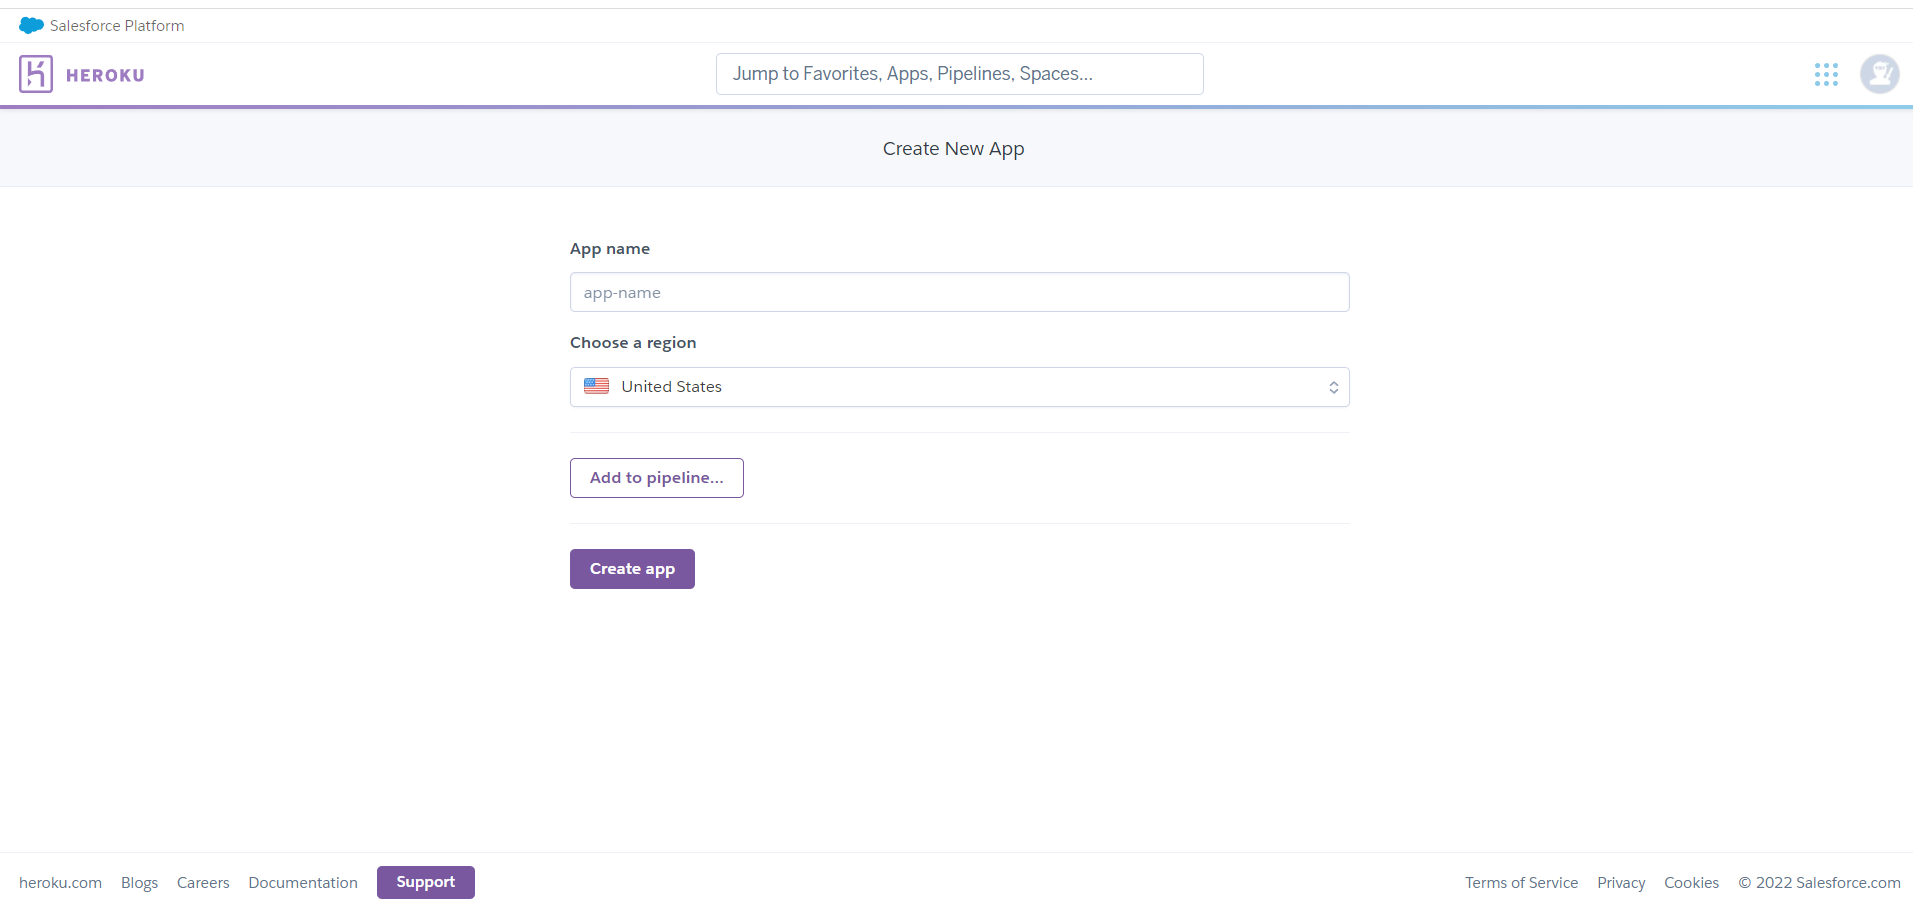
\includegraphics[scale=0.4]{slike/opis aplikacije.png} 
			 	\centering
			 	\caption{Opis aplikacije}
			 	\label{DS}
			 \end{figure} 
			 
			 Nakon upisivanja potrebnih informacija, dolazi se na početni prozor.
			 \begin{figure}[H]
			 	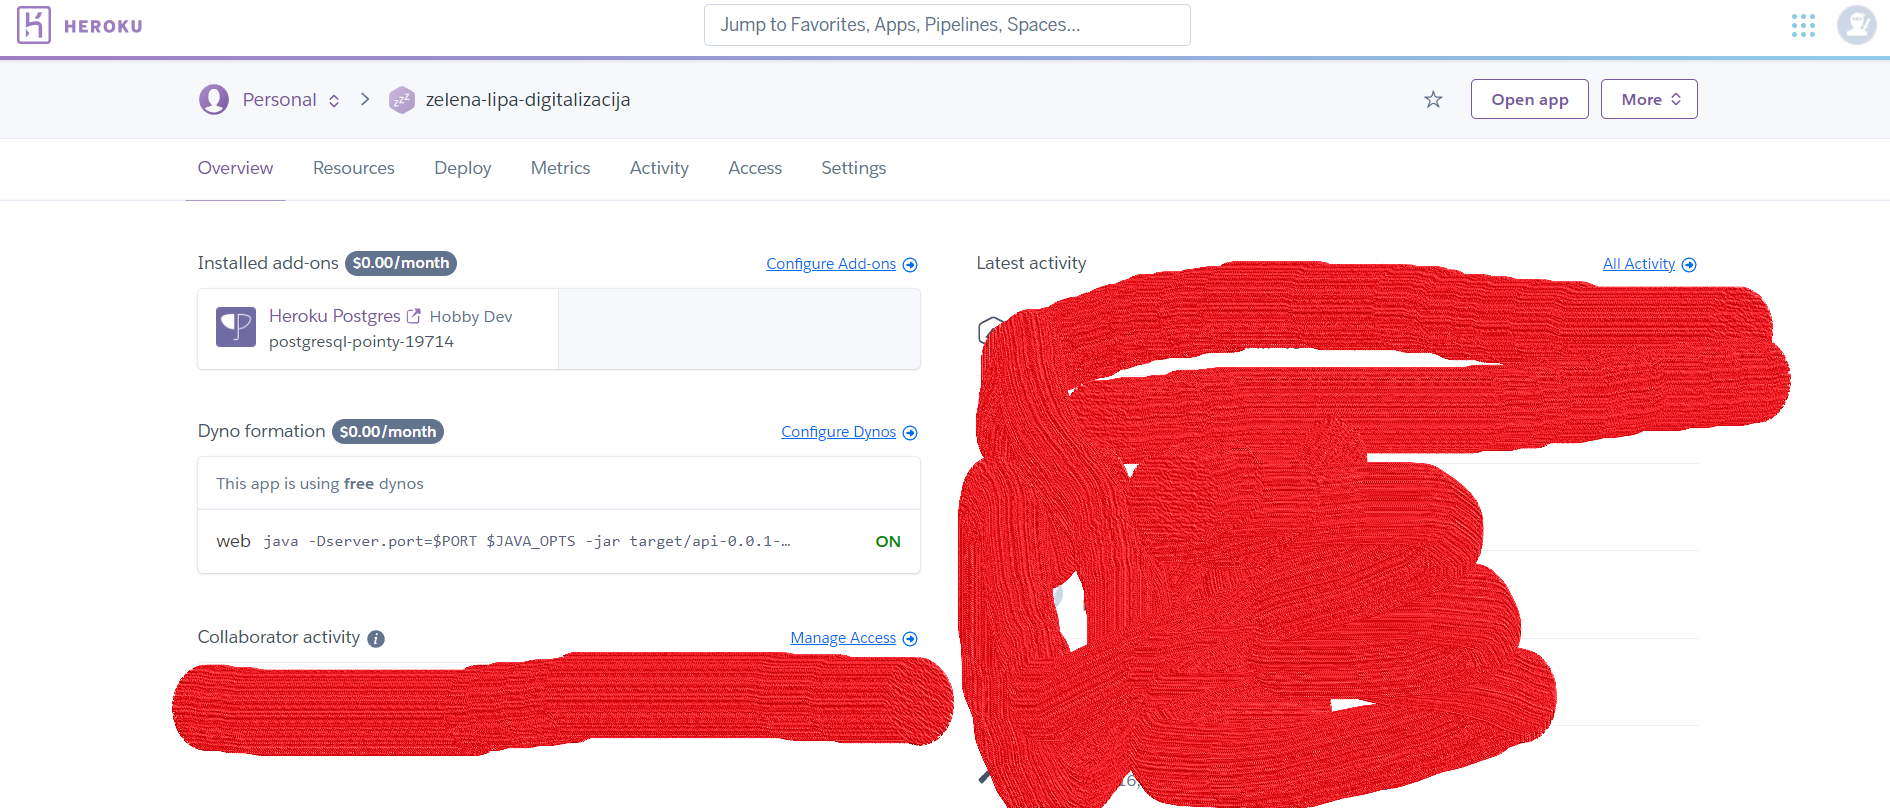
\includegraphics[scale=0.3]{slike/Overview.png} 
			 	\centering
			 	\caption{ Overview.}
			 	\label{DS}
			 \end{figure}
			 
			 Ovdje se pruža puno mogućnosti, a trenutno ćemo se fokusirati na Add-ons i dodat ćemo novi (besplatni) add-on Heroku Postgre. Sada imamo bazu podataka za našu aplikaciju.
			 
			 Sljedeće, na izborniku odabiremo Resources te pristupamo pojedinostima naše baze podataka klikom na Heroku Postgres.
			 
			 \begin{figure}[H]
			 	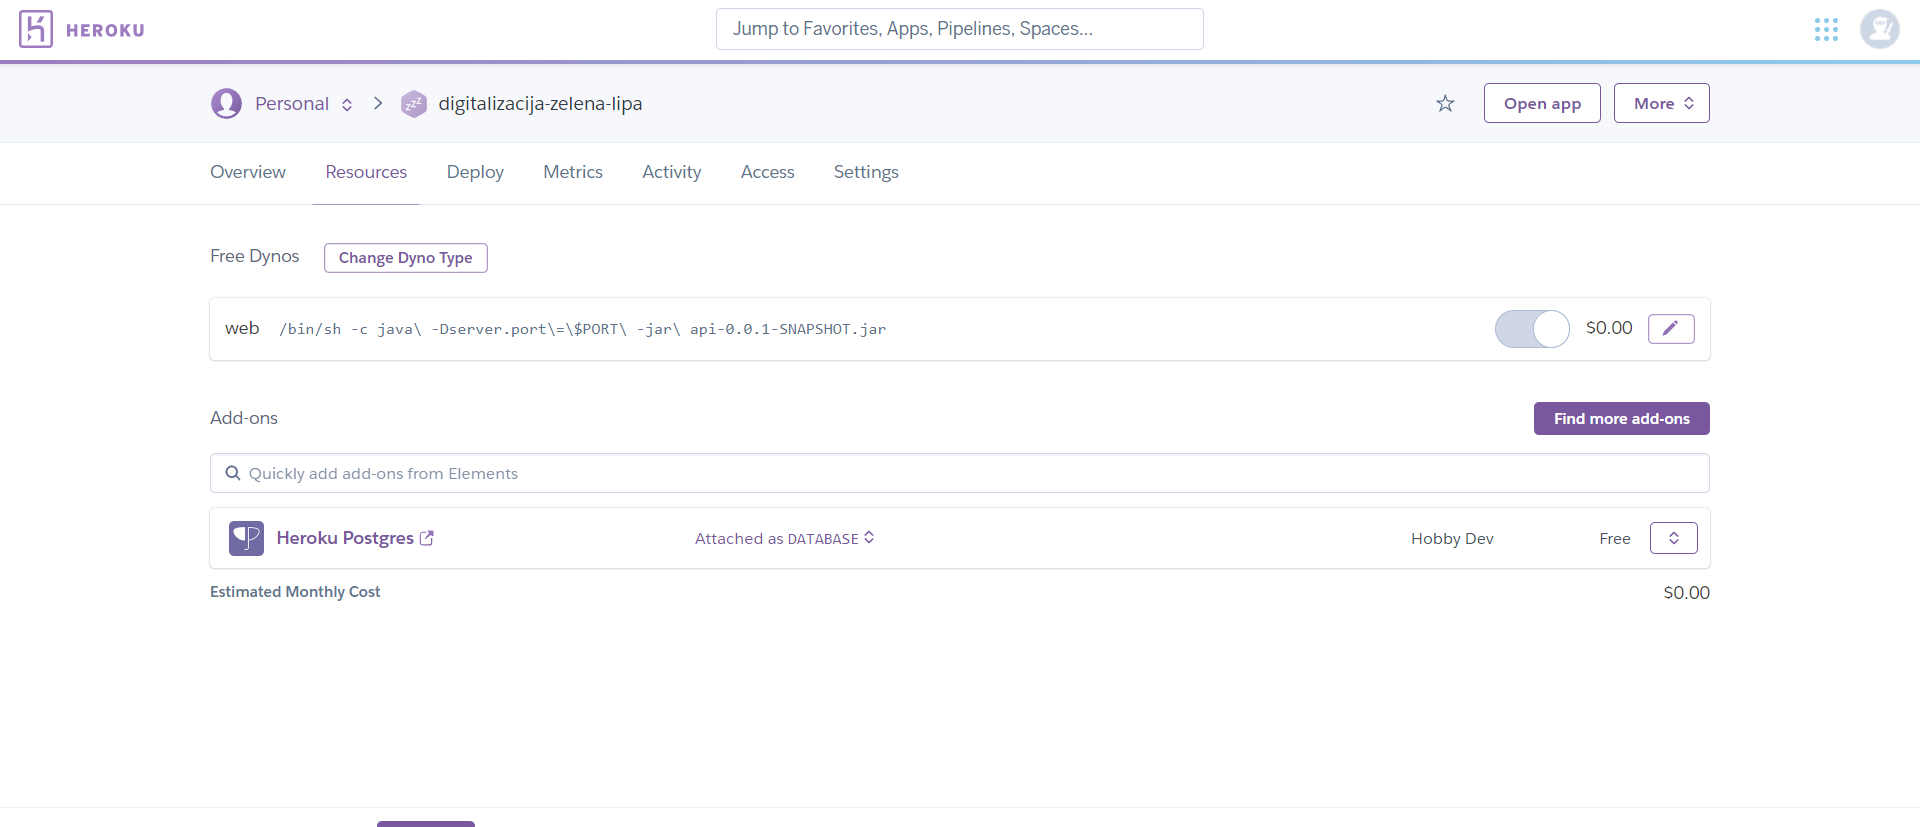
\includegraphics[scale=0.4]{slike/Resources.png} 
			 	\centering
			 	\caption{ Resources.}
			 	\label{DS}
			 \end{figure}
		 
		 Zatim dolazimo do sljedećeg prozora:
			 
			 \begin{figure}[H]
			 	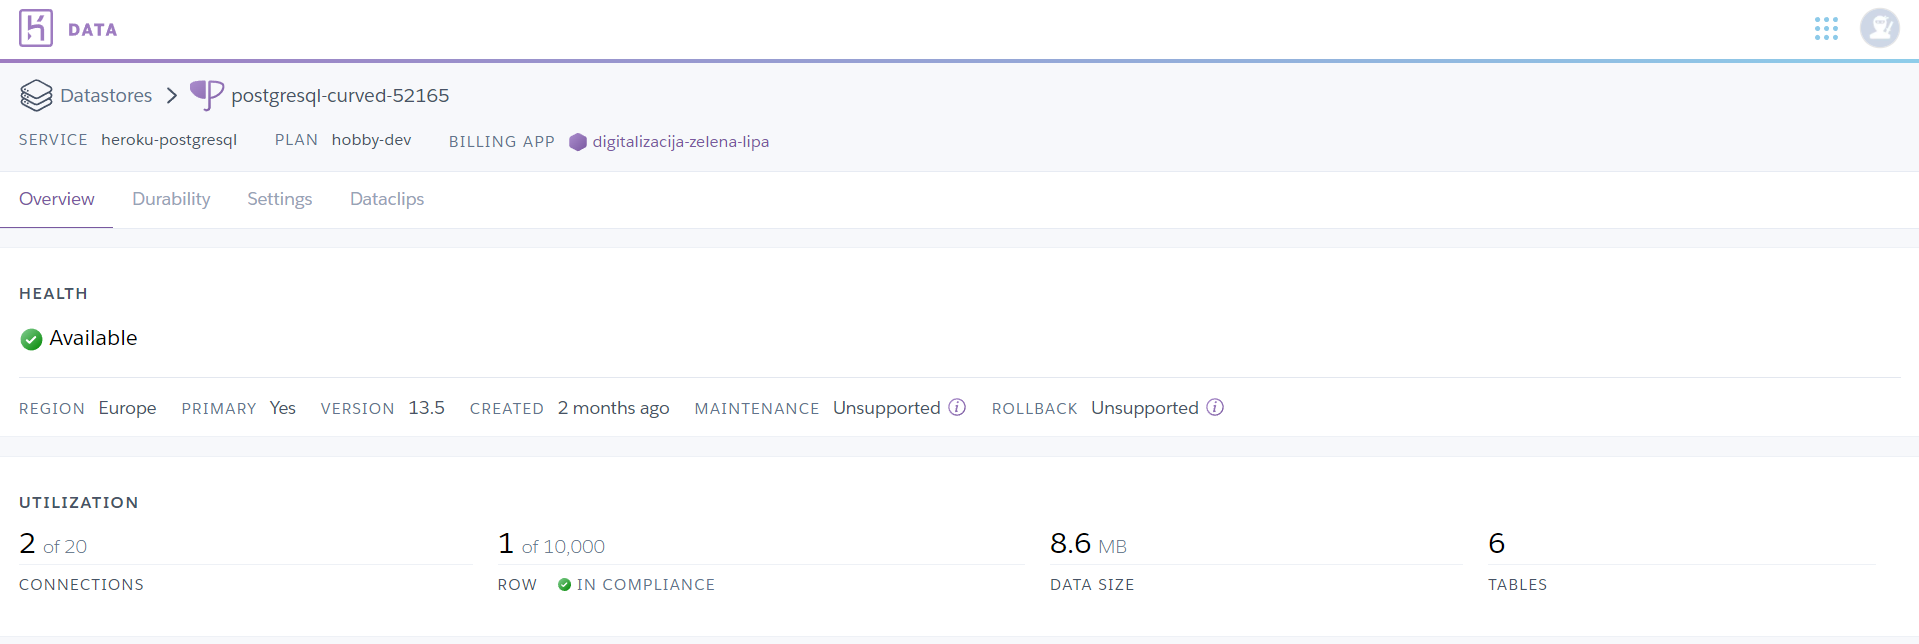
\includegraphics[scale=0.4]{slike/Datastores.png} 
			 	\centering
			 	\caption{ Database overview.}
			 	\label{DS}
			 \end{figure}
		 
		 	Odavde idemo na Settings.
		 	
		 	
		 	\begin{figure}[H]
		 		\includegraphics[scale=0.3]{slike/Datacredentials.png} 
		 		\centering
		 		\caption{ Database credentials.}
		 		\label{DS}
		 	\end{figure}
			 
			 U Database Creentials nam je prikazan user, pass, port, itd. Sve to će nam biti potrebno da bismo tu bazu mogli urediti i pripremiti za našu aplikaciju.
			 
			 Sada nam je potreban \textbf{PGadmin}, koji ćemo koristiti za pristupanje bazi podataka te unošenje. Instalacijski program se može preuzeti na ovom linku: \textit{https://www.postgresql.org/download/} Potrebno je odabrati odgovarajuću verziju za OS vlastitog računala. Nakon što se preuzme instalacijski program, potrebno ga je pokrenuti. Sada treba slijediti korake instalacije, odabir instalacijskog direktorija, odabrati komponente (preporučujemo da se označe sve 4), direktorij za podatke, lozinku (po želji), port (ostavite predložena 5432) i jezik. Možete pokrenuti instalaciju. Pri prvom pokretanju će se tražiti lozinka, koju je korisnik upisao pri instalaciji. Nakon verifikacije i ulaska u aplikaciju se već nalazi jedan napravljen server koji je lokalan te korisnik može graditi svoje baze podataka na njemu. Sada ćemo pažnju posvetiti tome kako se pristupa serveru koji drži našu bazu podataka za aplikaciju.
			 
			 Desnim klikom na padajući izbornik "Servers" se prikaže:
			 
			 \begin{figure}[H]
			 	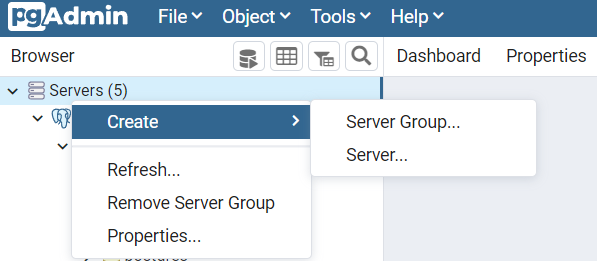
\includegraphics[scale=1]{slike/novi server.png} 
			 	\centering
			 	\caption{ Kreiranje novog servera.}
			 	\label{DS}
			 \end{figure}
		 	
		 	 Odabiremo Server i prelazimo na sljedeći prozor.
			 
			 Dolazimo do novog prozora "General" u kojem je potrebno proizvoljno nazvati server (u našem primjeru Server-alfa)
			 \begin{figure}[H]
			 	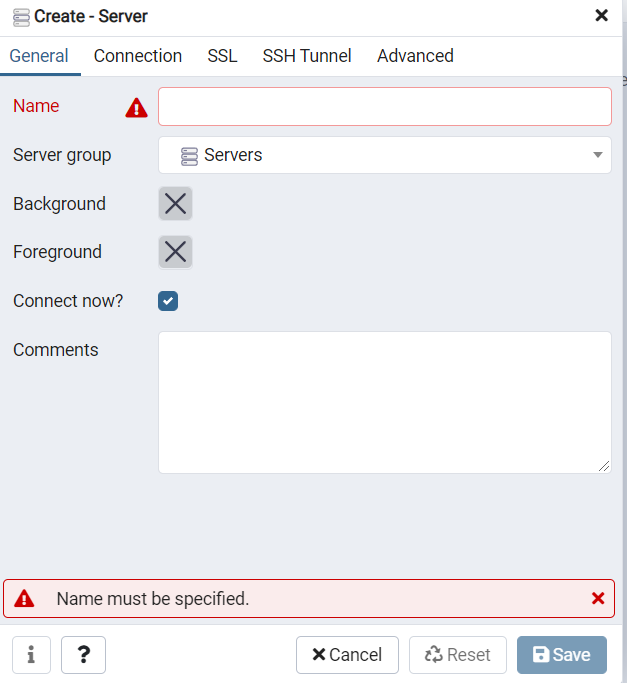
\includegraphics[scale=1]{slike/server general.png} 
			 	\centering
			 	\caption{ Server-General.}
			 	\label{DS}
			 \end{figure}
			 
			 Nakon toga prelazimo na "Connection". 
			 
			 \begin{figure}[H]
			 	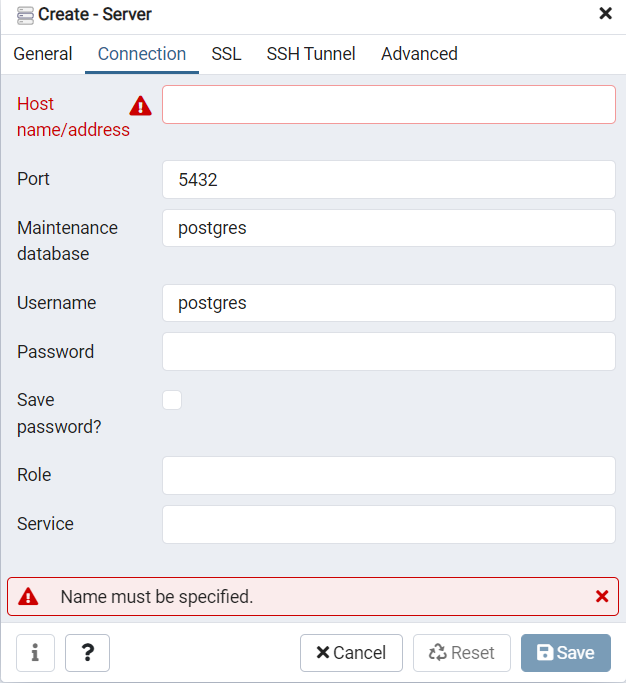
\includegraphics[scale=1]{slike/server connection.png} 
			 	\centering
			 	\caption{ Server-Connection.}
			 	\label{DS}
			 \end{figure}
			 
			 U novom prozoru je potrebno upisati sve što nam je ponuđeno na slici  "Database credentials". Pritiskom na gumb "Save" stvorili smo server na našem PGadminu te sada imamo pristup bazi podataka za našu heroku aplikaciju.
			 \begin{figure}[H]
			 	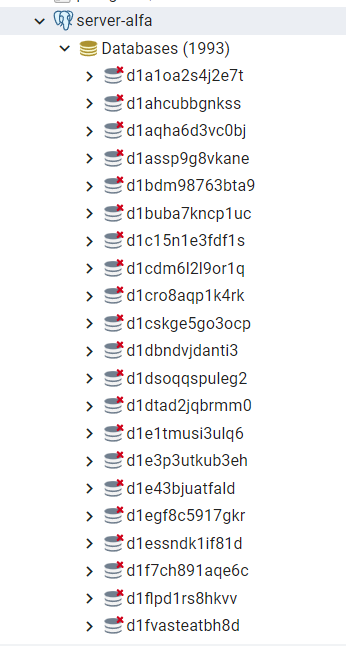
\includegraphics[scale=0.5]{slike/Server-alfa.png} 
			 	\centering
			 	\caption{ Izbornik bazi podataka.}
			 	\label{DS}
			 \end{figure}
			 
			 Ponuđeno je puno bazi podataka, ali pristup je dozvoljen samo bazi za našu aplikaciju.
			  \begin{figure}[H]
			 	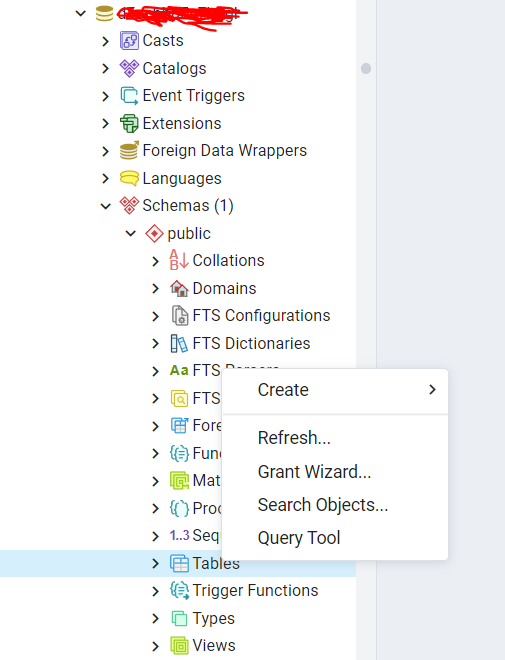
\includegraphics[scale=0.7]{slike/baza.png} 
			 	\centering
			 	\caption{ Izbornik naše baze podataka.}
			 	\label{DS}
			 \end{figure}
			 
			 Odaberemo sad Query tool kao što je prikazano na Slici. Otvorit će se prostor za uređivanje teksta u kojem se upisuje kod za stvaranje tablica, umetanje podataka u te tablice i sve drugo što je potrebno za uređivanje baze. Pokretanjem koda se gradi baza i spremna je za korištenje. 
			 
			 Sada kada smo pripremili bazu potrebno je završni kod staviti na git od naše heroku aplikacije, vraćamo se ponovno na naš račun.
			 
			 Odabiremo Deploy.
			 \begin{figure}[H]
			 	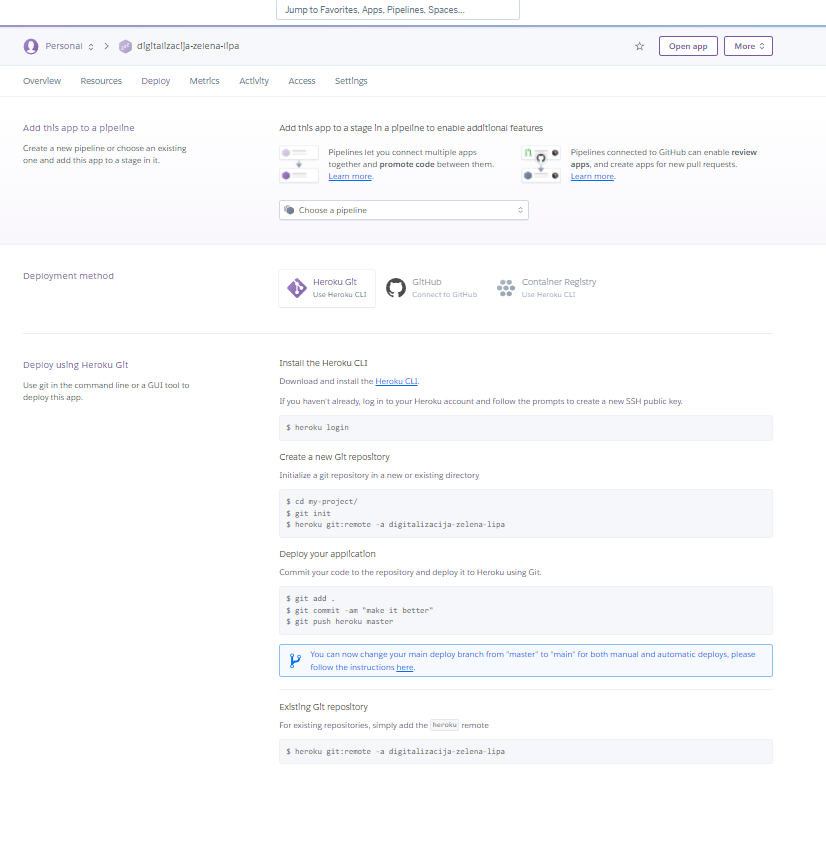
\includegraphics[scale=0.7]{slike/Deploy.png} 
			 	\centering
			 	\caption{ Deploy.}
			 	\label{DS}
			 \end{figure}
			 
			 Ovdje se nalazi uputa od preuzimanju Heroku CLI i opis kako klonirati git repozitorij te kako staviti završni kod na repozitorij. Naredbom git push heroku master vaš kod se stavlja na repozitorij i automatski pokreće te će vam u terminalu pisati link na kojem je vaša web aplikacija, kojoj možete pristupiti sa svog browsera i početi koristiti.
			 \eject
			 
			 \textbf{Dodatak:}
			 
			 U našoj aplikaciji, heroku nije mogao podržati funkcionalnost OCR (Tesseract) dokumenata. Pokušali smo s build-packageom za Tesseract koji je ponuđen u Heroku, što nije pomoglo. Iako bi sve funkcioniralo lokalno, nikako nismo mogli namjestiti da heroku pronađe knjižnice (engl. library) za Tesseract OCR. Da bi ipak omogućili našoj aplikaciji da izvodi OCR morali smo dodati docker container (https://devcenter.heroku.com/articles/build-docker-images-heroku-yml) koji je osigurao da su potrebne knjižnice za OCR instalirane te da im naša aplikacija može pristupiti.
			 
			 
			
			
			 
			
			
			\eject 